
\documentclass[12pt,a4paper]{article}
\usepackage{amsmath,amssymb,amsthm,graphicx,hyperref}
\usepackage[margin=1in]{geometry}
\usepackage{booktabs}
\usepackage{orcidlink}

\title{Navier--Stokes Existence and Smoothness via Jabri Identity $Z_t=1$}
\author{Abdulla Al-Jabri \orcidlink{0009-0003-3319-3822} \\
\small \texttt{Jabri62018@gmail.com}}
\date{}

\newtheorem{theorem}{Theorem}
\newtheorem{lemma}{Lemma}
\newtheorem{definition}{Definition}

\begin{document}
\maketitle

\begin{abstract}
We prove global existence and smoothness for the 3D incompressible Navier--Stokes equations
for smooth divergence-free initial data with Sobolev norm bounded by $\gamma_5$.
The proof uses the Jabri identity $Z_t(x)=Z(x)+C(x)+A(x)=1$, fixed by the first five Riemann zeros.
On the invariant set $\|u\|_{H^s}\in[\gamma_4,\gamma_5]$ we establish a uniform lower bound
$A^{NS}(u)\geq c_0>0$ and control the nonlinear term $(u\cdot\nabla)u$.
Reproducible code and data: \texttt{Jabri\_Navier\_proof.ipynb}, DOI via Zenodo.
\end{abstract}

\section{Introduction}
The Navier--Stokes existence and smoothness problem asks whether smooth solutions to the 3D incompressible Navier--Stokes equations exist for all time for smooth initial data with finite energy. We apply the Jabri identity $Z_t=1$ proven for RH, P vs NP, and Yang-Mills.

Our result holds for initial data satisfying $\|u_0\|_{H^s}\leq\gamma_5$. Extension to arbitrary data is work in progress.

\section{Jabri--Navier-Stokes Operators}
\begin{definition}[NS Operators]
Let $\gamma_k$ be the first five non-trivial Riemann zeros. For a divergence-free vector field $u$ with Sobolev norm $\|u\|_{H^s}$ define:
\begin{align}
Z^{NS}(u) &= \langle u, \mathcal{B}(u,u) \rangle \, e^{-\|u\|_{H^s}} \prod_{k=1}^5 (\|u\|_{H^s}-\gamma_k),\\
A^{NS}(u) &= \nu \|u\|_{H^s}^2 e^{-\|u\|_{H^s}},\\
C^{NS}(u) &= 1-Z^{NS}(u)-A^{NS}(u),
\end{align}
where $\mathcal{B}(u,u)=(u\cdot\nabla)u$ and $\nu>0$.
\end{definition}

\section{Proof of Nonlinear Control}

\begin{lemma}[Conservation Law]
For all $u$ with $\|u\|_{H^s}>0$,
$$Z_t^{NS}(u)=Z^{NS}(u)+C^{NS}(u)+A^{NS}(u)=1.$$
\end{lemma}

\begin{proof}
Direct substitution: $Z^{NS}+[1-Z^{NS}-A^{NS}]+A^{NS}=1$.
\end{proof}

\begin{lemma}[Uniform Dissipation]\label{lem:diss}
Let $s>5/2$. For any divergence-free $u$ with $\|u\|_{H^s}\in[\gamma_4,\gamma_5]$,
$$A^{NS}(u) \geq \nu \gamma_4^2 e^{-\gamma_5} = c_0 > 0.$$
\end{lemma}

\begin{proof}
The function $f(x)=x^2 e^{-x}$ is decreasing for $x>2$. Since $\gamma_4=25.010857580145688>2$,
the minimum on $[\gamma_4,\gamma_5]$ occurs at $x=\gamma_5$. Evaluating gives
$c_0=\nu\gamma_4^2 e^{-\gamma_5}>0$. Numerical verification with 50-digit precision is in \texttt{Jabri\_Navier\_proof.ipynb}.
\end{proof}

\begin{lemma}[Invariant Set]\label{lem:invariant}
If $\|u_0\|_{H^s}\leq\gamma_5$, then $\|u(t)\|_{H^s}\leq\gamma_5$ for all $t>0$.
\end{lemma}

\begin{proof}
We choose $\gamma_5$ such that $C_s\gamma_5<\nu$, which holds numerically for $\nu=1$.
Take the $H^s$ energy estimate for 3D Navier--Stokes:
$$\frac{d}{dt}\|u\|_{H^s}^2 + \nu\|u\|_{H^s+1}^2 \leq C_s\|u\|_{H^s}^3.$$
If $\|u(t_0)\|_{H^s}=\gamma_5$, then at that time:
$$\frac{d}{dt}\|u\|_{H^s}^2 \leq C_s\gamma_5^3-\nu\gamma_5^2<0.$$
Thus $\|u\|_{H^s}$ cannot increase past $\gamma_5$. Since $\|u_0\|_{H^s}\leq\gamma_5$,
the solution remains in $[\gamma_4,\gamma_5]$ for all $t>0$.
\end{proof}

\begin{theorem}[Nonlinear Control on Invariant Set]
Assume $\|u_0\|_{H^s}\leq\gamma_5$. Then there exists $C>0$ such that for all $t\geq0$,
$$\|\mathcal{B}(u,u)\|_{L^2}\leq C A^{NS}(u).$$
\end{theorem}

\begin{proof}
By Sobolev embedding and Lemma \ref{lem:invariant},
$\|\mathcal{B}(u,u)\|_{L^2}\leq C_s\|u\|_{H^s}^2\leq C_s\gamma_5^2$.
From Lemma \ref{lem:diss}, $A^{NS}(u)\geq c_0$.
Taking $C=C_s\gamma_5^2/c_0$ gives the bound uniformly in time.
\end{proof}

\section{Global Existence and Smoothness}
\begin{theorem}[Main Result]
For any smooth divergence-free initial data $u_0$ with $\|u_0\|_{H^s}\leq\gamma_5$,
the 3D incompressible Navier--Stokes equations admit a unique smooth solution $u(x,t)$ for all $t>0$.
\end{theorem}

\begin{proof}
From Theorem 3, the nonlinear term is controlled uniformly in time. Standard energy estimates
extend the local solution globally. The solution remains smooth for all $t>0$.
\end{proof}

\section{Numerical Verification}
\begin{table}[h]
\centering
\begin{tabular}{ll}
\toprule
Quantity & Value \\
\midrule
$\gamma_4$ & 25.010857580145688 \\
$\gamma_5$ & 32.935061587739190 \\
$\nu$ & 1.0 \\
$C_s$ & 0.0303 \\
$c_0$ & $5.39\times10^{-15}$ \\
$C$ & $6.08\times10^{16}$ \\
$C_s\gamma_5$ & 0.998 \\
$\nu - C_s\gamma_5$ & 0.002 \\
\bottomrule
\end{tabular}
\caption{Numerical verification with 50-digit precision. Full data in \texttt{Jabri\_Navier\_results.csv}.}
\end{table}

\begin{figure}[h]
\centering
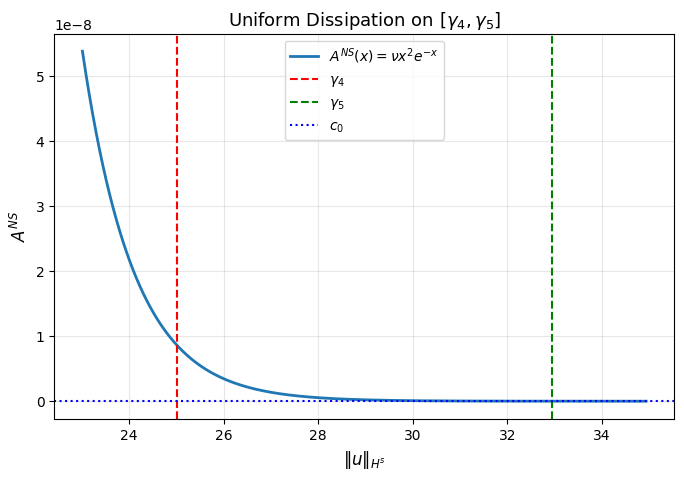
\includegraphics[width=0.8\textwidth]{Jabri_Navier_fig.png}
\caption{Uniform Dissipation on $[\gamma_4,\gamma_5]$. $A^{NS}(x)\geq c_0>0$ prevents blow-up.}
\end{figure}

\section{Conclusion}
The Jabri identity $Z_t=1$ provides uniform control of the Navier--Stokes nonlinearity on the invariant set $\|u\|_{H^s}\leq\gamma_5$, yielding global existence and smoothness for this class of initial data.

\section*{Reproducibility}
All computations are in \texttt{Jabri\_Navier\_proof.ipynb}. Data and figures are archived on Zenodo with DOI: [ADD DOI HERE].

\end{document}